\chapter{Firewalls, IDS and Web Security}
\section{Firewalls}
A firewall is an integrated collection of security measures designed to prevent unauthorized electronic access to a networked computer system. A network firewall is similar to firewalls in building construction, because in both cases they are intended to isolate one "network" or "compartment" from another.
\subsection{Policies}
To protect private networks and individual machines from the dangers of the greater Internet, a firewall can be employed to filter incoming or outgoing traffic based on a predefined set of rules called firewall policies.
Packets flowing through a firewall can have one of three outcomes:
\begin{itemize}
\item \textbf{Accepted}: permitted through the firewall
\item \textbf{Dropped}: not allowed through with no indication of failure
\item  \textbf{Rejected}: not allowed through, accompanied by an attempt to inform the source that the packet was rejected
\end{itemize}
Policies used by the firewall to handle packets are based on several properties of the packets being inspected, including the protocol used, such as:
\begin{itemize}
\item TCP or UDP
\item the source and destination IP addresses
\item the source and destination ports
\item the application-level payload of the packet (e.g., whether it contains a virus)
\end{itemize}
\subsubsection{Blacklist and Whitelist}
There are two fundamental approaches to creating firewall policies (or rulesets) to effectively minimize vulnerability to the outside world while maintaining the desired functionality for the machines in the trusted
internal network (or individual computer):
\begin{itemize}
\item \textbf{Blacklist approach}: All packets are allowed through except those that fit the rules defined
specifically in a blacklist. This type of configuration is more flexible in ensuring that service to the internal network is not disrupted by the firewall, but is naïve from a security perspective in that it assumes the network administrator can enumerate all of the properties of malicious traffic.
\item \textbf{Whitelist approach}: A safer approach to defining a firewall ruleset is the default-deny policy, in which packets are dropped or rejected unless they are specifically allowed by the firewall.
\end{itemize}
\subsection{Firewall types}
\begin{itemize}
\item \textbf{packet filters (stateless)}: If a packet matches the packet filter's set of rules, the packet filter will drop or accept it. 
\item \textbf{"stateful" filters}: It maintains records of all connections passing through it and can determine if a packet is either the start of a new connection, a part of an existing connection, or is an invalid packet.
\item \textbf{application layer}: It works like a proxy so it can “understand” certain applications and protocols. It may inspect the contents of the traffic, blocking what it views as inappropriate content (i.e. websites, viruses, vulnerabilities, ...).
\end{itemize}
\subsubsection{Stateless firewalls (Packet filters)}
A stateless firewall doesn't maintain any remembered context (or “state”) with respect to the packets it is processing. Instead, it treats each packet attempting to travel through it in isolation without considering packets that it has processed previously. \\
\textbf{Security Note:} Stateless firewalls may have to be fairly restrictive in order to prevent most attacks.
\subsubsection{Stateful firewalls}
Stateful firewalls can tell when packets are part of legitimate sessions originating within a trusted network. They
maintain tables containing information on each active connection, including the IP addresses, ports, and sequence numbers of packets.\\
\textbf{Security Note:} Using these tables, stateful firewalls can allow only inbound TCP packets that are in response to a connection initiated from within the internal network.
\section{Tunnels}
The contents of TCP packets are not normally encrypted, so if someone is eavesdropping on a TCP connection, he can often see the complete contents of the payloads in this session. One way to prevent such eavesdropping without
changing the software performing the communication is to use a tunneling protocol.\\
In such a protocol, the communication between a client and server is automatically encrypted, so that useful eavesdropping is infeasible. Packets sent over the Internet are automatically encrypted.
\section{Intrusion Detection Systems (IDS)}
An intrusion detection system (IDS) is a device or software application that monitors network or system activities for malicious activities or policy violations and produces reports to a management station. \\
Some definition:
\begin{itemize}
\item \textbf{Intrusion}: Actions aimed at compromising the security of the target (confidentiality, integrity, availability of computing/networking resources)
\item \textbf{Intrusion detection}: The identification through intrusion signatures and report of intrusion activities
\item \textbf{Intrusion prevention}: The process of both detecting intrusion activities and managing automatic responsive actions throughout the network
\end{itemize}
\subsection{IDS Components}
The \textbf{IDS manager} compiles data from the \textbf{IDS sensors} to determine if an intrusion has occurred. This determination is based on a set of site policies, which are rules and conditions that define probable intrusions. If an IDS manager detects an intrusion, then it sounds an alarm.
\begin{figure}[htbp]
	\centering
	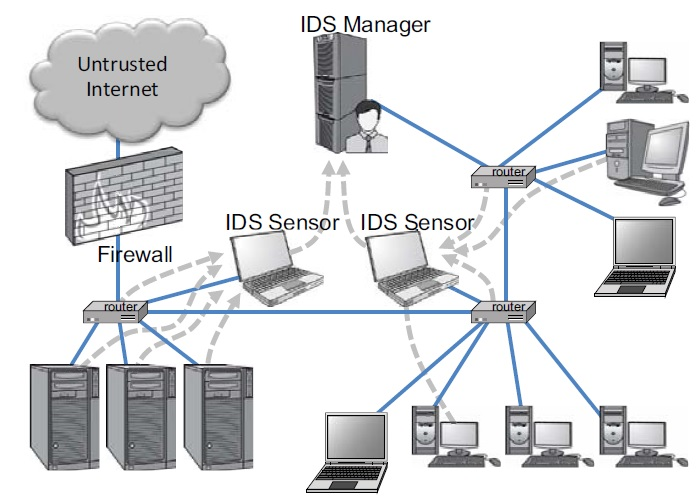
\includegraphics[width=0.5\linewidth]{Immagini/firewalls/IDS.png}
	\caption{IDS Components} 	
	\label{fig:IDS_components}
\end{figure}
\subsection{Intrusions}
An IDS is designed to detect a number of threats, including the following:
\begin{itemize}
\item \textbf{Masquerader}: an attacker who is falsely using the identity and/or credentials of a legitimate user to gain access to a computer system or network
\item \textbf{Misfeasor}: a legitimate user who performs actions he is not authorized to do 
\item \textbf{Clandestine user}: a user who tries to block or cover up his actions by deleting audit files and/or system logs
\end{itemize}
In addition, an IDS is designed to detect automated attacks and threats, including the following:
\begin{itemize}
\item \textbf{Port scans}: information gathering intended to determine which ports on a host are open for TCP connections
\item \textbf{Denial-of-service attacks}: network attacks meant to overwhelm a host and shut out legitimate accesses
\item \textbf{Malware attacks}: replicating malicious software attacks, such as Trojan horses, computer worms, viruses, etc.
\item \textbf{ARP spoofing}: an attempt to redirect IP traffic in a local-area network
\item \textbf{DNS cache poisoning}: a pharming attack directed at changing a host's DNS cache to create a falsified domain-name/IP-address association
\end{itemize}
\subsection{IDS Data} 
In an influential 1987 paper, Dorothy Denning identified several fields that should be included in IDS event records:
\begin{itemize}
\item \textbf{Subject}: the initiator of an action on the target
\item \textbf{Object}: the resource being targeted, such as a file, command, device, or network protocol
\item \textbf{Action}: the operation being performed by the subject towards the object
\item \textbf{Exception-condition}: any error message or exception condition that was raised by this action
\item \textbf{Resource-usage}: quantitative items that were expended by the system performing or responding to this action
\item \textbf{Time-stamp}: a unique identifier for the moment in time when this action was initiated
\end{itemize}
\subsection{Types of Intrusion Detection Systems} 
\subsubsection{Rule-Based Intrusion Detection} 
Rules identify the types of actions that match certain known profiles for an intrusion attack, in which case the rule would encode a signature for such an attack. Thus, if the IDS manager sees an event that matches the signature for such a rule, it would immediately sound an alarm, possibly even indicating the particular type of attack that is suspected.
\subsubsection{Statistical Intrusion Detection}
A profile is built, which is a statistical representation of the typical ways that a user acts or a host is used; hence, it can be used to determine when a user or host is acting in highly unusual, anomalous ways.
Once a user profile is in place, the IDS manager can determine thresholds for anomalous behaviors and then sound an alarm any time a user or host deviates significantly from the stored profile for that person or machine.
\section{Cross Site Scripting (XSS)}
Cross-site scripting is a type of computer security vulnerability typically found in Web applications. XSS enables attackers to \textbf{inject client-side script} into Web pages viewed by other users. It can be used for many types of attack: phishing, hijacking, changing of user settings, cookie theft/poisoning, false advertising, execution of code on the client, etc. 
\begin{figure}[htbp]
	\centering
	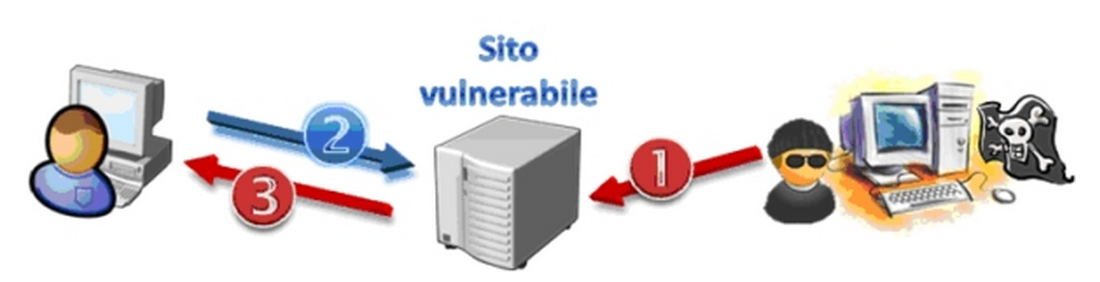
\includegraphics[width=0.5\linewidth]{Immagini/firewalls/XSS.png}
	\caption{Schema base di un attacco XSS} 	
	\label{fig:XSS_attack}
\end{figure}
\\
Methods for injecting malicious code are of three types:
\begin{itemize}
	\item \textbf{DOM-based (“type 0”)}: The attacker stores the malicious code locally in a standard object model for representing HTML or XML called the Document Object Model or DOM for short.
	\item \textbf{Reflected XSS (“type 1”)}: the attack script is reflected back to the user as part of a page from the victim site.
	\item \textbf{Stored XSS (“type 2”)}: the attacker stores the malicious code in a resource managed by the web application, such as a database.
\end{itemize}
Possible client-side XSS defenses are the following:
\begin{itemize}
	\item \textbf{Proxy-based}: analyze the HTTP traffic exchanged between user's web browser and the target web server by scanning for special HTML characters and encoding them before executing the page on the user's web browser (i.e. NoScript -	Firefox plugin).
	\item \textbf{Application-level firewall}: analyze browsed HTML pages for hyperlinks that might lead to leakage of sensitive information and stop bad requests using a set of connection rules.
	\item \textbf{Auditing system}: monitor execution of JavaScript code and compare the operations against high-level policies to detect malicious behavior.
\end{itemize}

\section{SQL Injection Attack}
Many web applications take user input from a form. Often this user input is used literally in the construction of a SQL query submitted to a database. For example:
\begin{lstlisting}
SELECT user 
FROM table
WHERE name = 'user input name'
\end{lstlisting}
A SQL injection attack involves placing SQL statements in the user input.
\subsubsection{Login Query: username and password} 
Here follows a standard query to check if the Login is correct:
\begin{lstlisting}
SELECT * 
FROM users 
WHERE user = '$usern' AND pwd = '$password'
\end{lstlisting}
If an attacker enter values for username/password as:
\begin{lstlisting}
$usern = "M' OR '1=1"
$password = "M' OR '1 = 1"
\end{lstlisting}
The resulting query will be:
\begin{lstlisting}
SELECT * 
FROM users 
WHERE user = 'M' OR '1=1' AND pwd = 'M' OR '1=1'
\end{lstlisting}
Result: you obtain the access!\\
Another query:
\begin{lstlisting}
SELECT user, pwd 
FROM users 
WHERE user = '$usern' 
\end{lstlisting}
If again:
\begin{lstlisting}
$usern = "M' OR '1=1" 
\end{lstlisting}
Result: you obtain the entire table!\\
To overcome this type of attack we have to check whether the result is one tuple only and the formal correctness of the result. \\
\linebreak
Considering another kind of malicious input, if there was:  
\begin{lstlisting} 
$usern="M' ; drop table user;"
\end{lstlisting}
Then we can use an \textbf{Escape method}, where all "malicious" characters will be changed.
Here it is shown an example: the following expression
\begin{lstlisting} 
Escape("t ' c") 
\end{lstlisting}
gives as a result:
\begin{lstlisting} 
"t \' c"
\end{lstlisting}
So, writing:
\begin{lstlisting} 
SELECT user, pwd 
FROM users 
WHERE user = '$usern'
\end{lstlisting}
and:
\begin{lstlisting} 
$usern = escape("M' ;drop table user;")
\end{lstlisting}
Gives, as result, the safe query:
\begin{lstlisting} 
SELECT user, pwd 
FROM users 
WHERE user='M\'drop table user;\''
\end{lstlisting}
\textbf{Solution} for SQL injection attack are: \textbf{Escape string} and \textbf{strict type verification}